\pagestyle{hedra}
\label{hedra}

\begin{textblock*}{5.625in}(0pt,0pt)%
\vspace*{-2.5cm}
\hspace*{-1.95cm}\includegraphics*[width=147mm]{./imgs/HEDRA.png}
\end{textblock*}

\pagebreak


\hspace{.5cm}

\begin{center}
\hspace*{-4.5cm}\raisebox{5.8cm}{\rotatebox[origin=t]{90}{\Formular{\textbf{Lançamento}}}}
\hspace*{4cm}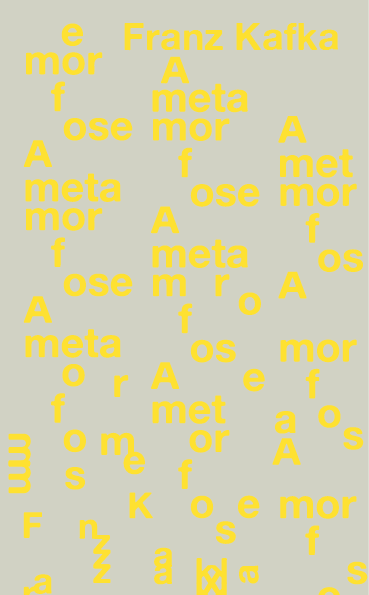
\includegraphics[width=45mm]{./imgs/kafka.png}
\end{center}

\hspace*{-7cm}\hrulefill\hspace*{-7cm}

\medskip

\noindent{}Obra mais famosa de Franz Kafka, {\slsc{A metamorfose}} dispensa apresentações. A história da transformação de Gregor Samsa é um clássico porque condensa perfeitamente as características da prosa kafkiana, este conceito que se torna importante na nossa repertoriação do mundo: kafkiano é, pois, o contraditório da nossa cultura ocidental desumanizada, em que o irracional é criado justamente pelas estruturas burocráticas ultrarracionalizadas.

%\hspace{.5cm}
\vfill

\hspace*{-.4cm}\begin{minipage}[c]{1\linewidth}
\small{
{\Formular{\textbf{
\hspace*{-.1cm}Título: A metamorfose [bilíngue]\\
Autor: Franz Kafka\\ 
Páginas: 196\\
Formato: 13x21cm\\
Preço: R\$ 39,90\\
ISBN: 978-85-7715-601-6\\
Disponibilidade: Em breve
}}}}
\end{minipage}


\pagebreak

\hspace{.5cm}

\begin{center}
\hspace*{-.5cm}
\includegraphics[width=43.7mm]{./imgs/maquiavel.jpeg}
\end{center}

\hspace*{-7cm}\hrulefill\hspace*{-7cm}

\medskip

\noindent{}{\slsc{O príncipe}} ganha sua mais completa edição bilíngue, trazendo ao leitor brasileiro contato com a melhor edição do texto original italiano --- a Edição Crítica Inglese ---, acrescida de introdução e notas explicativas. Obra mais emblemática de Nicolau Maquiavel, {\slsc{O príncipe}} assinala uma nova forma de analisar a política, marcada principalmente pelo realismo que procura apreender a política como ela é --- em sua prática terrena.

%\hspace{.5cm}
\vfill

\hspace*{-.4cm}\begin{minipage}[c]{1\linewidth}
\small{
{\Formular{\textbf{
\hspace*{-.1cm}Título: O príncipe [bilíngue]\\
Autor: Nicolau Maquiavel\\ 
Páginas: 508\\
Formato: 13x21cm\\
Preço: R\$ 49,90\\
ISBN: 978-85-7715-604-7\\
Disponibilidade: Em breve
}}}}
\end{minipage}

\pagebreak

\hspace{.5cm}

\begin{center}
\hspace*{-4.5cm}\raisebox{5.5cm}{\rotatebox[origin=t]{90}{\Formular{\textbf{Lançamento}}}}
\hspace*{4cm}
\includegraphics[width=43mm]{./imgs/wwb.jpg}
\end{center}

\hspace*{-7cm}\hrulefill\hspace*{-7cm}

\medskip

\noindent{}Romancista, dramaturgo, historiador e militante abolicionista, William Wells Brown tem em sua {\slsc{Narrativa autobiográfica}} um dos mais importantes romances afro"-americanos da história. A obra reconta os horrores da escravidão, percorrendo o tráfico interno de escravos nos \scalebox{.8}{EUA} e a relação de Brown com seus donos e familiares, destacando assim a individualidade e que se desenvolveu sob uma instituição totalizante e desumanizadora.

%\hspace{.5cm}
\vfill

\hspace*{-.4cm}\begin{minipage}[c]{1\linewidth}
\small{
{\Formular{\textbf{
\hspace*{-.1cm}Título: Narrativa de William Wells Brown, escravo fugitivo, escrita por ele mesmo\\
Autor: William Wells Brown\\ 
Páginas: 142\\
Formato: 14x21cm\\
Preço: R\$ 39,90\\
ISBN: 978-85-7715-618-4\\
Disponibilidade: Em breve
}}}}
\end{minipage}

\pagebreak

\hspace{.5cm}

\begin{center}
\hspace*{-.5cm}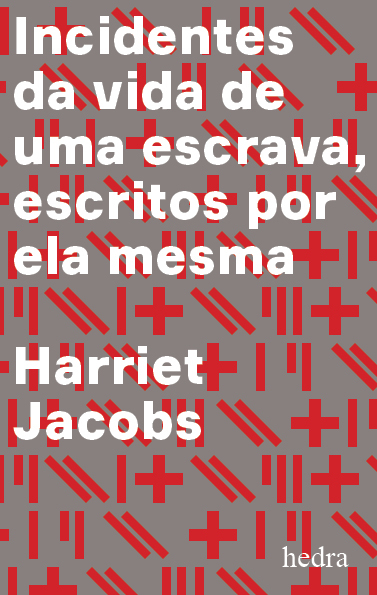
\includegraphics[width=43.4mm]{./imgs/jacobs.jpg}
\end{center}

\hspace*{-7cm}\hrulefill\hspace*{-7cm}

\medskip

\noindent{}Nascida na Carolina do Norte, por volta do outono de 1813, Harriet Ann Jacobs viveu intensamente a tragédia da escravidão, e dela resulta este relato cru, de prosa vívida e dramática que, sem deixar de se inserir no corpus dos relatos da escravidão norte"-americana, é pioneiro e inspirador das autobiografias femininas, e joga luz no perverso sistema de assédio e coação que era partilhado apenas entre as mulheres.

%\hspace{.5cm}
\vfill

\hspace*{-.4cm}\begin{minipage}[c]{1\linewidth}
\small{
{\Formular{\textbf{
\hspace*{-.1cm}Título: Incidentes da vida de uma escrava, escritos por ela mesma\\
Autor: Harriet Jacobs\\ 
Páginas: 406\\
Formato: 14x21cm\\
Preço: R\$ 49,90\\
ISBN: 978-85-7715-617-7\\
Disponibilidade: Em breve
}}}}
\end{minipage}


\pagebreak

\hspace{.5cm}

\begin{center}
\hspace*{-4.5cm}\raisebox{5.5cm}{\rotatebox[origin=t]{90}{\Formular{\textbf{Lançamento}}}}
\hspace*{4cm}
\includegraphics[width=43mm]{./imgs/wpa.jpg}
\end{center}

\hspace*{-7cm}\hrulefill\hspace*{-7cm}

\medskip

\noindent{}{\slsc{Nascidos na escravidão}} resulta de um amplo esforço de tomar depoimentos de ex"-escravos dos Estados Unidos, totalizando 2400 narrativas inéditas, das quais a edição reúne 204, em uma curadoria por tema que permite entrever a memória das milhares de pessoas sobreviventes do trauma do cativeiro, em sua complexidade, e desmontar certos mitos correntes sobre a escravidão através de depoimentos em primeira mão.


%\hspace{.5cm}
\vfill

\hspace*{-.4cm}\begin{minipage}[c]{1\linewidth}
\small{
{\Formular{\textbf{
\hspace*{-.1cm}Título: Nascidos na escravidão: depoimentos norte"-americanos\\
Autor: Paul D. Escott (org.)\\ 
Páginas: 348\\
Formato: 14x21cm\\
Preço: R\$ 49,90\\
ISBN: 978-85-7715-619-1\\
Disponibilidade: Em breve
}}}}
\end{minipage}

\pagebreak

\hspace{.5cm}

\begin{center}
\hspace*{-.5cm}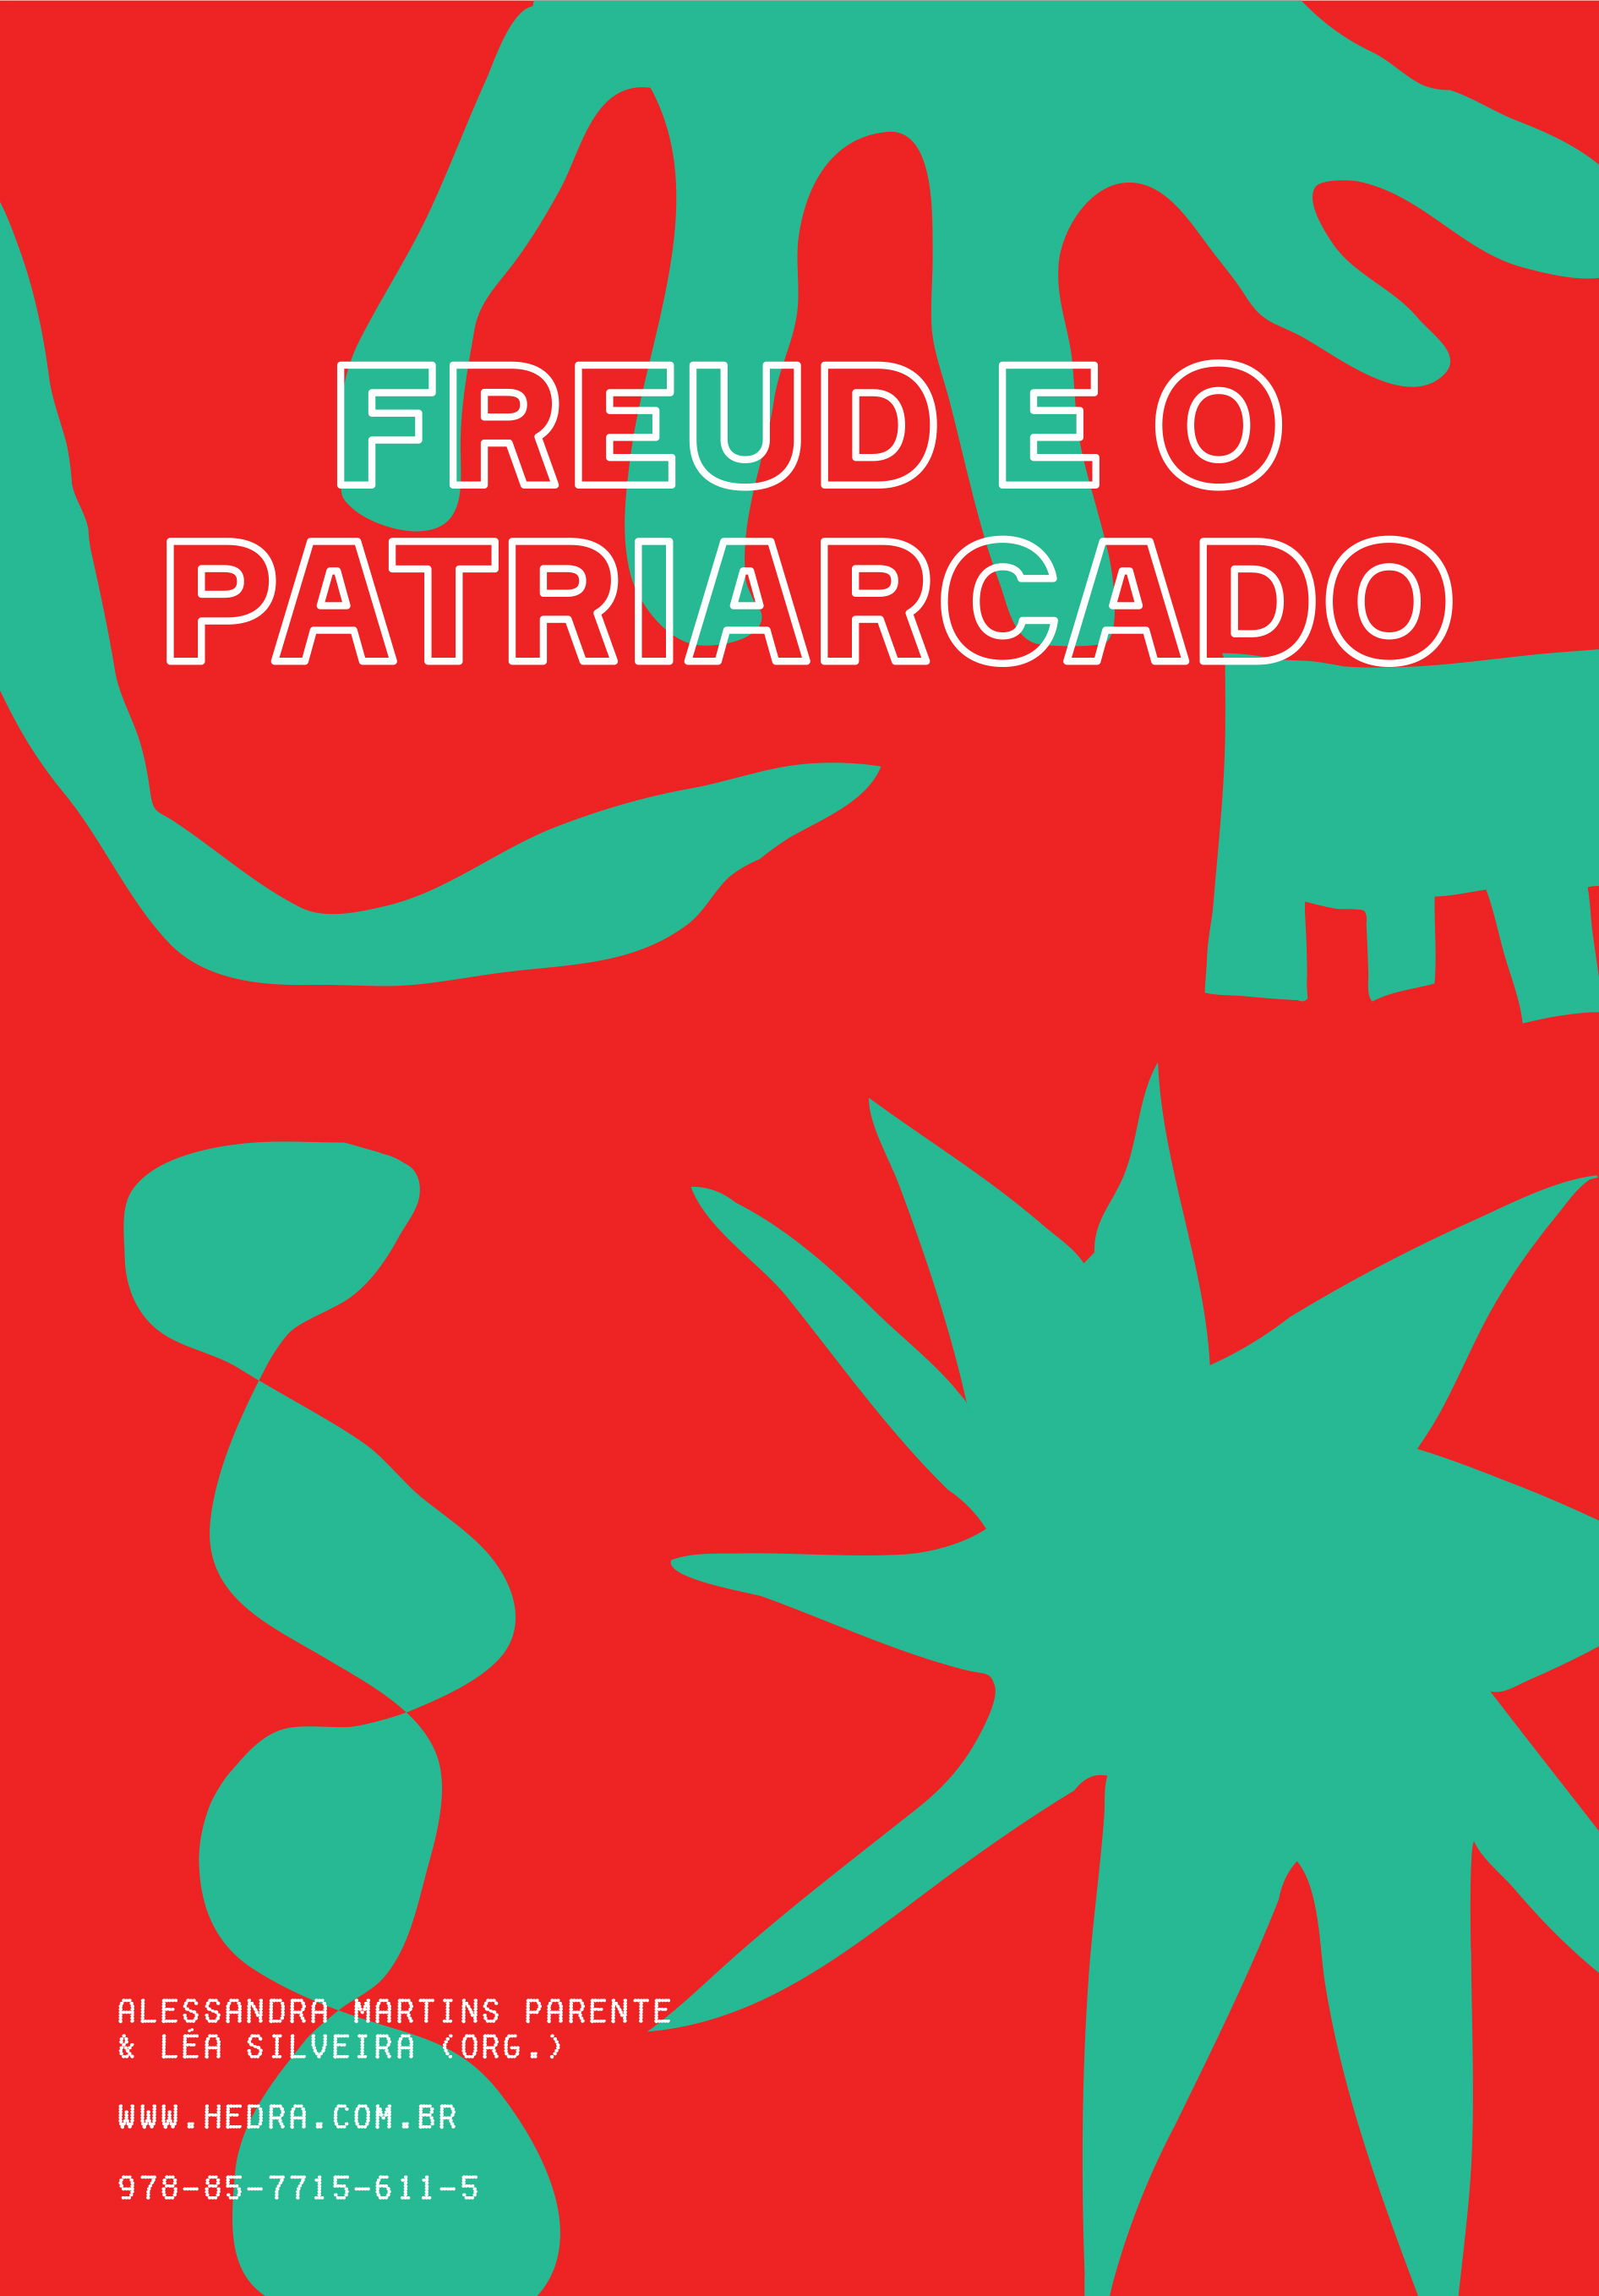
\includegraphics[width=68.5mm]{./imgs/freud.jpg}
\end{center}

\hspace*{-7cm}\hrulefill\hspace*{-7cm}

\medskip

\noindent{}{\slsc{Freud e o patriarcado}} parte da constatação de que o campo da teoria psicanalítica põe em jogo uma forma de conceber o psíquico que assume, em seu centro, uma equivalência generalizada entre cultura, civilização e masculinidade, algo que, para as autoras e os autores de {\slsc{Freud e o patriarcado}}, deveria ser explicado, não dado. Sobre essa trilha, trata"-se de explorar a legitimidade dos modelos freudianos, seja preservando"-os ou repensando"-os.

%\hspace{.5cm}
\vfill

\hspace*{-.4cm}\begin{minipage}[c]{1\linewidth}
\small{
{\Formular{\textbf{
\hspace*{-.1cm}Título: Freud e o patriarcado\\
Autor: Alessandra Martins Parente e Léa Silveira (org.)\\ 
Páginas: 398\\
Formato: 16x23cm\\
Preço: R\$ 64,90\\
ISBN: 978-85-7715-611-5\\
Disponibilidade: Disponível a partir de abril
}}}}
\end{minipage}

\pagebreak

\hspace{.5cm}

\begin{center}
\hspace*{-3cm}\raisebox{5.5cm}{\rotatebox[origin=t]{90}{\Formular{\textbf{Lançamento}}}}
\hspace*{3cm}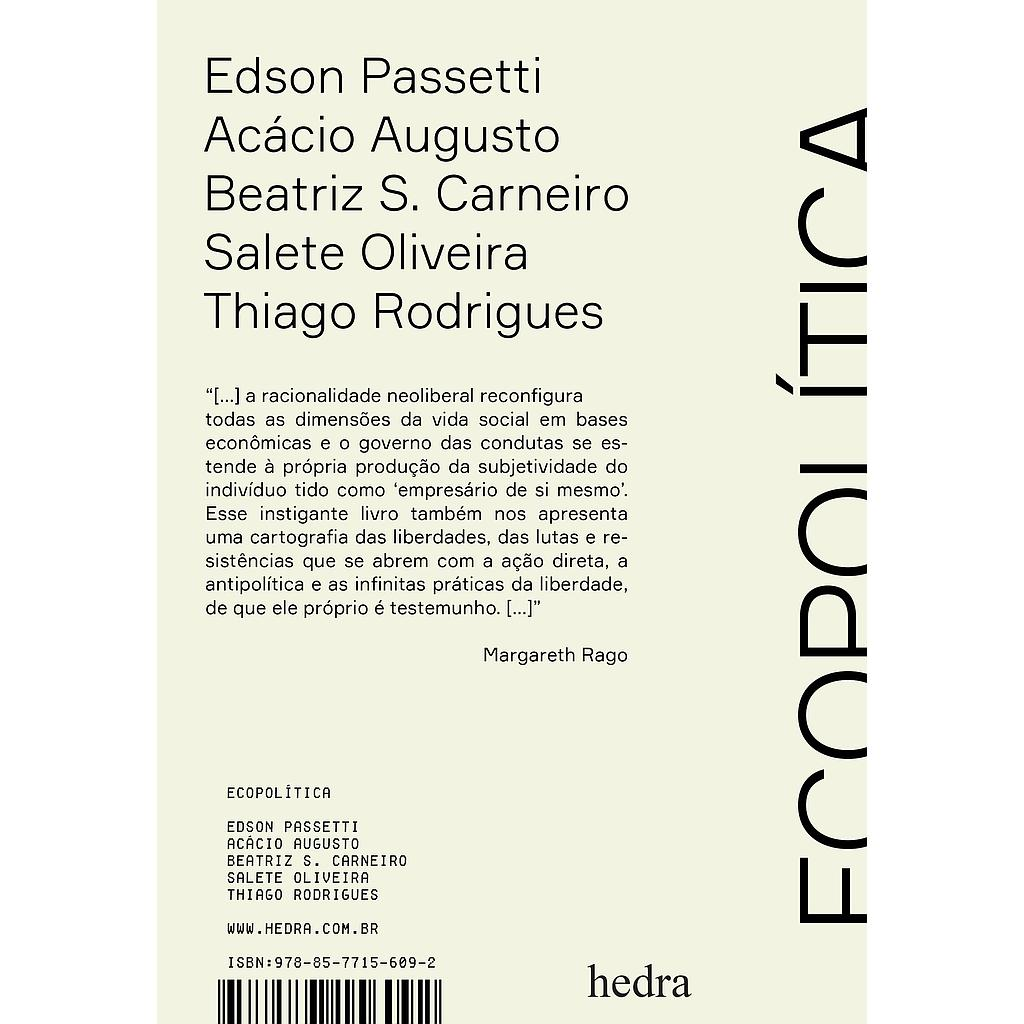
\includegraphics[width=70mm]{./eco.jpeg}
\end{center}

\hspace*{-7cm}\hrulefill\hspace*{-7cm}

\medskip

\noindent{}{\slsc{Ecopolítica}} mapeia a passagem da biopolítica — o controle da vida analisado por Foucault — para a ecopolítica, nova forma de governar que emerge pós-\scalebox{.8}{II} Guerra Mundial e se estende a todas as esferas do mundo natural. Os estudiosos do grupo Nu"-Sol percorrem e analisam acontecimentos históricos e contemporâneos, e atravessam fluxos de poder para conclamar à criação de resistências libertárias e esquivas às globalizantes linhas de controle.

%\hspace{.5cm}
\vfill

\hspace*{-.4cm}\begin{minipage}[c]{1\linewidth}
\small{
{\Formular{\textbf{
\hspace*{-.1cm}Título: Ecopolítica\\
Autor: Edson Passetti (org.)\\ 
Páginas: 476\\
Formato: 16x23cm\\
Preço: R\$ 79,90\\
ISBN: 978-85-7715-609-2\\
Disponibilidade: Disponível
}}}}
\end{minipage}

\pagebreak

\hspace{.5cm}

\begin{center}
\hspace*{-.5cm}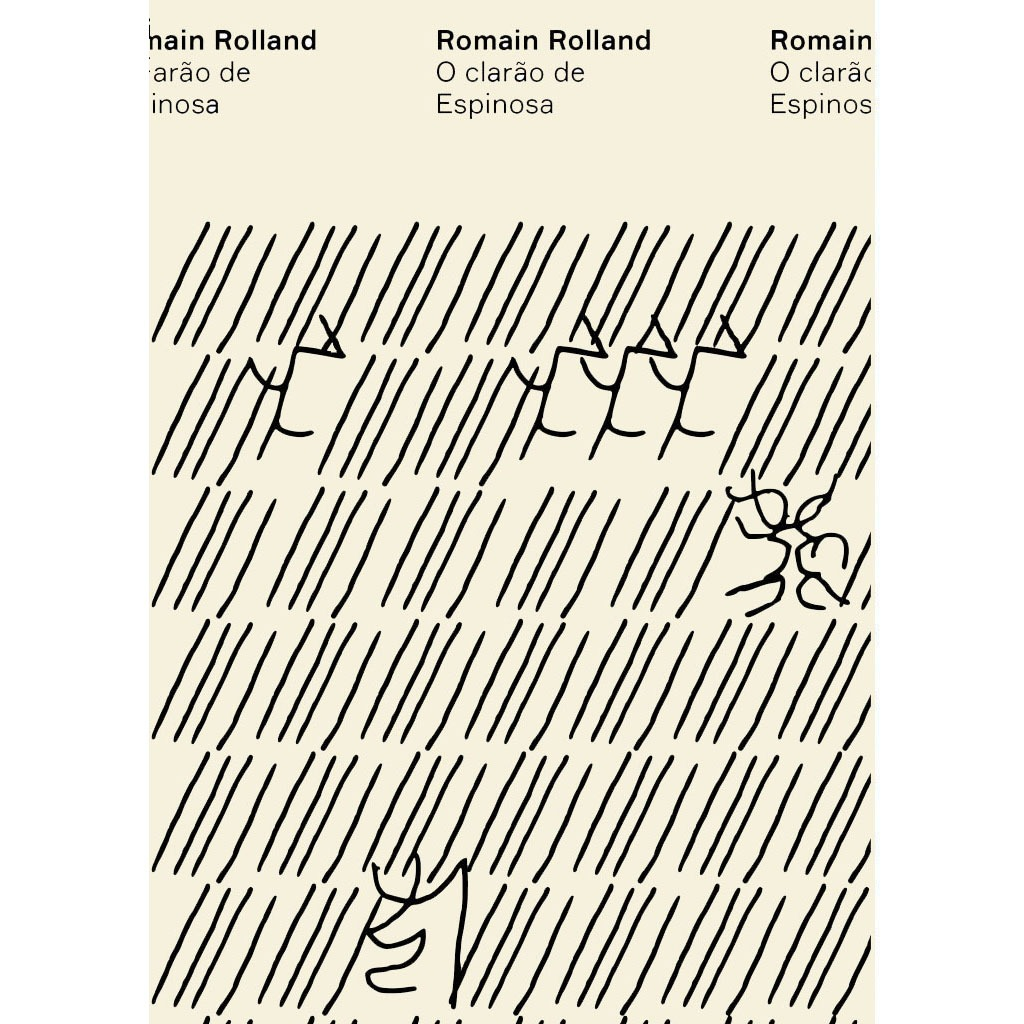
\includegraphics[width=70mm]{./grid/romain.jpeg}
\end{center}

\hspace*{-7cm}\hrulefill\hspace*{-7cm}

\medskip

\noindent{}Romain Rolland (1866-1944) novelista, biógrafo e músico francês (Nobel de 1915) escreveu estas páginas sobre Espinosa, que fazem parte de {\slsc{Confissões inéditas}}, capítulo do livro intitulado {\slsc{A viagem interior}} (1942) . Neste pequeno trecho o adolescente Romain Rolland conta o “clarão” que teve em sua vida ao ler Espinosa pela primeira vez aos 16 anos e como isso definiu sua vida e carreira.

\vfill

\hspace*{-.4cm}\begin{minipage}[c]{1\linewidth}
\small{
{\Formular{\textbf{
\hspace*{-.1cm}Título: O clarão de Espinosa\\
Autor: Romain Rolland\\ 
Páginas: 57\\
Formato: 11x18cm\\
Preço: R\$ 29,90\\
ISBN: 978-65-8109-708-0\\
Disponibilidade: Em breve
}}}}
\end{minipage}

\pagebreak

\hspace{.5cm}

\begin{center}
\hspace*{-3cm}\raisebox{5.5cm}{\rotatebox[origin=t]{90}{\Formular{\textbf{Lançamento}}}}
\hspace*{3cm}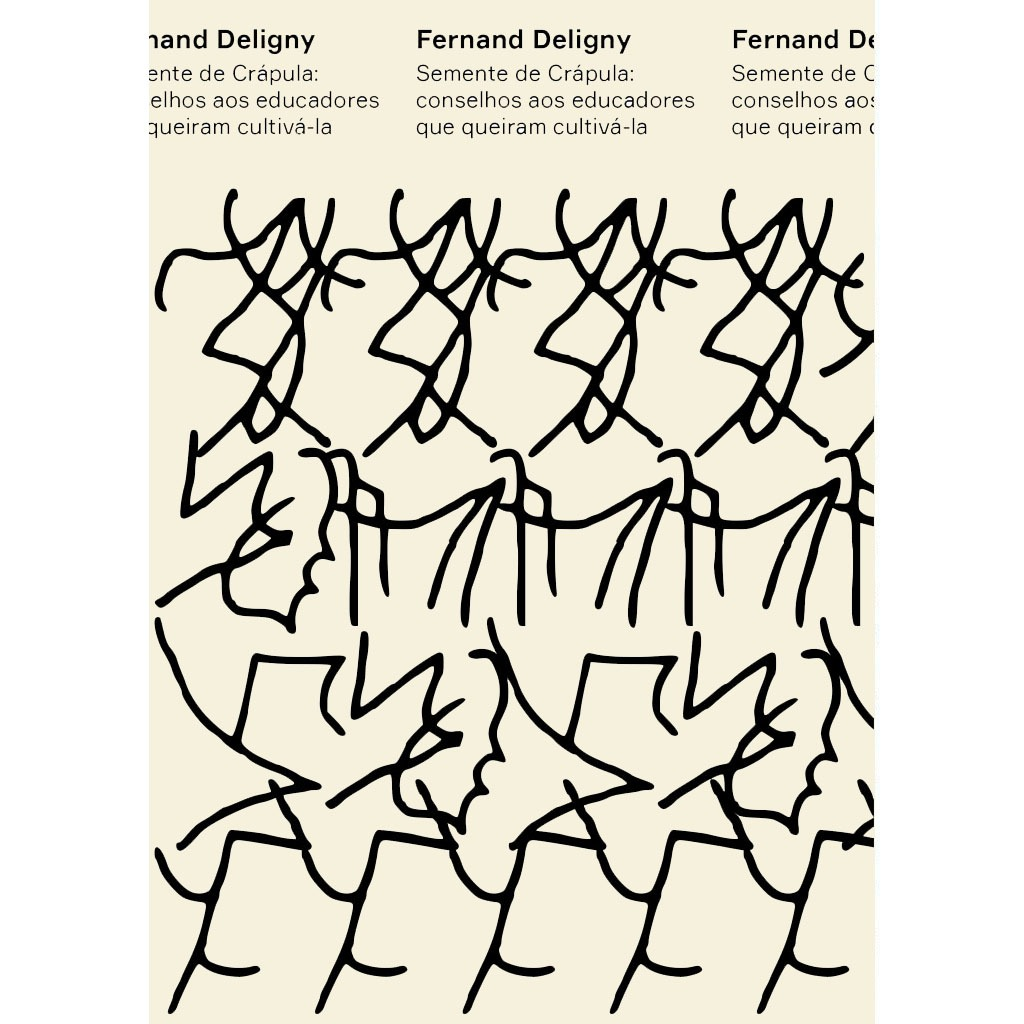
\includegraphics[width=70mm]{./grid/deligny.jpeg}
\end{center}

\hspace*{-7cm}\hrulefill\hspace*{-7cm}

\medskip

\noindent{}{\slsc{Semente de crápula}} é o primeiro livro de Fernand Deligny e um balizador do seu trabalho que o situaria enquanto uma das maiores referências da educação especial. Em belos aforismas, as sementes de que aqui se trata são de jovens, cultivados pelo educador que deve deixar de lutar contra as ervas daninhas, pragas sociais atadas ao nosso convívio social, para mergulhar nas dinâmicas espaciais dos jovens.

\vfill

\hspace*{-.4cm}\begin{minipage}[c]{1\linewidth}
\small{
{\Formular{\textbf{
\hspace*{-.1cm}Título: Semente de crápula: conselhos aos educadores que queiram cultivá-la\\
Autor: Fernand Deligny\\ 
Páginas: 96\\
Formato: 11x18cm\\
Preço: R\$ 34,90\\
ISBN: 978-65-8109-709-7\\
Disponibilidade: Em breve
}}}}
\end{minipage}

\pagebreak

\hspace{.5cm}

\begin{center}
\hspace*{-.5cm}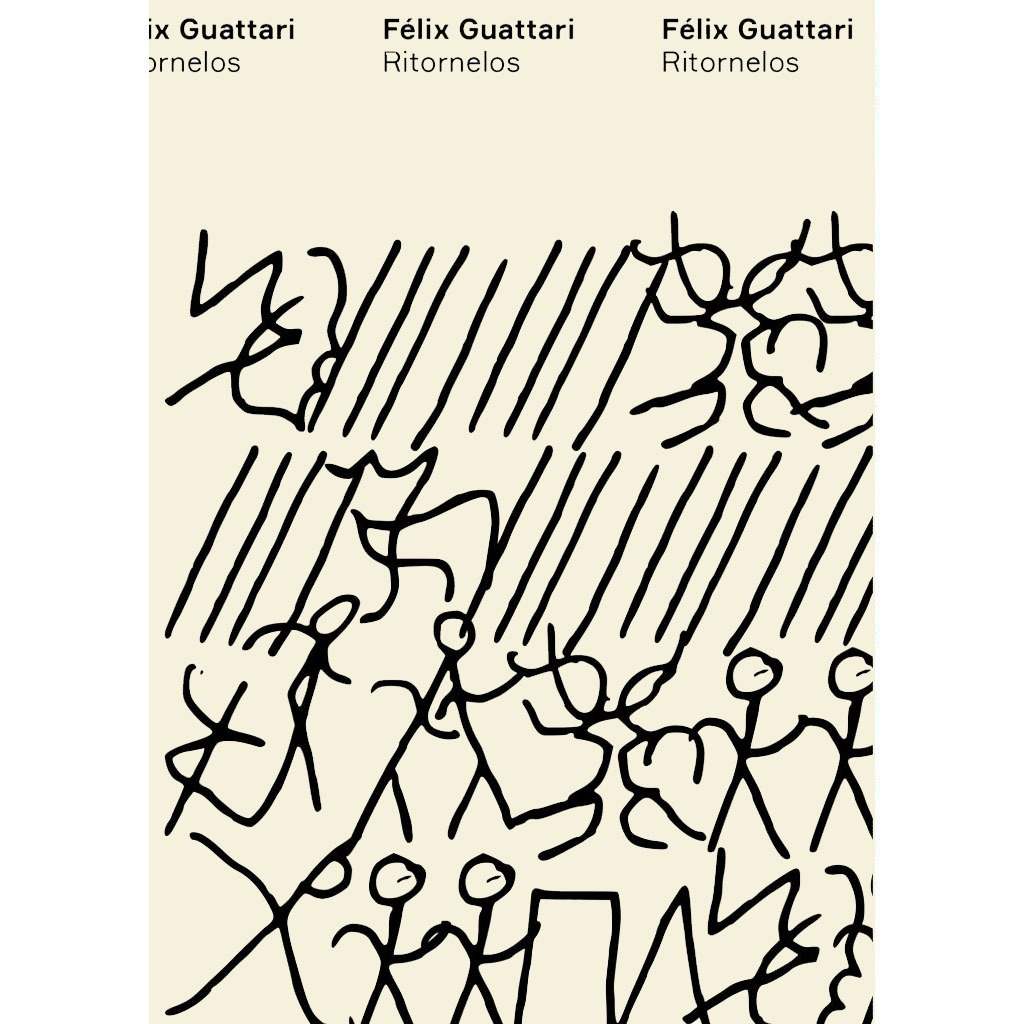
\includegraphics[width=70mm]{./grid/guattari.jpeg}
\end{center}

\hspace*{-7cm}\hrulefill\hspace*{-7cm}

\medskip

\noindent{}Livro póstumo do pensador e psicanalista Félix Guattari, {\slsc{Ritornelos}} é inclassificável. Misto de poesia, relatos autobiográficos, frames do cotidiano, toda potência da escrita esquiza irrompe nessas páginas de alta voltagem poética e imagética. Além de arguto intelectual, Guattari aparece em {\slsc{Ritornelos}} enquanto poeta sensível aos instantâneos e surreais quadros da vida.

\vfill

\hspace*{-.4cm}\begin{minipage}[c]{1\linewidth}
\small{
{\Formular{\textbf{
\hspace*{-.1cm}Título: Ritornelos\\
Autor: Félix Guattari\\ 
Páginas: 134\\
Formato: 11x18cm\\
Preço: R\$ 40,00\\
ISBN: 978-65-8109-702-8\\
Disponibilidade: Disponível
}}}}
\end{minipage}

\pagebreak

\hspace{.5cm}

\begin{center}
\hspace*{-3cm}\raisebox{5.5cm}{\rotatebox[origin=t]{90}{\Formular{\textbf{Lançamento}}}}
\hspace*{3cm}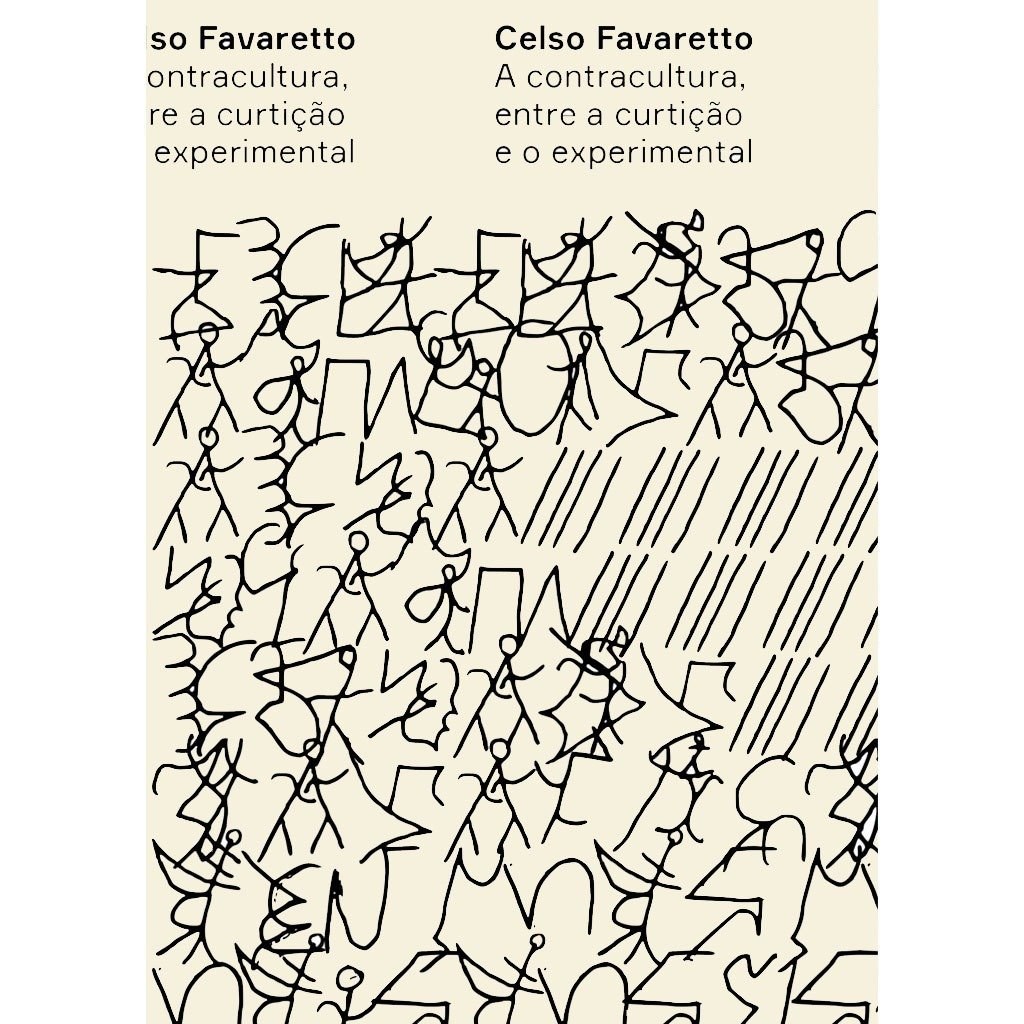
\includegraphics[width=70mm]{./grid/favaretto.jpeg}
\end{center}

\hspace*{-7cm}\hrulefill\hspace*{-7cm}

\medskip

\noindent{}Em {\slsc{Contracultura}}, Celso Favaretto aborda as manifestações que marcaram a produção artística brasileira entre os anos 60 e 70. Manifestava"-se então uma nova sensibilidade, que explorava as possibilidades abertas pelo tropicalismo. Para o autor, longe de um suposto “vazio cultural”, a contracultura, em suas expressões, definiu comportamentos e experimentações de grande vitalidade, inclusive como resistência à cultura oficial e à ditadura.

\vfill

\hspace*{-.4cm}\begin{minipage}[c]{1\linewidth}
\small{
{\Formular{\textbf{
\hspace*{-.1cm}Título: A contracultura, entre a curtição e o experimental\\
Autor: Celso Favaretto\\ 
Páginas: 142\\
Formato: 11x18cm\\
Preço: R\$ 40,00\\
ISBN: 978-65-8109-703-5\\
Disponibilidade: Disponível
}}}}
\end{minipage}

\pagebreak
\pagestyle{hedracat}

\begin{multicols}{2}
\begin{enumerate}
\item Ecopolítica, {\Formular{\textbf{Edson Passetti (org.)}}}	
\item Mare nostrum: Paranã Tipi, {\Formular{\textbf{Fabio Atui}}}
\item Crônicas de caça e criação, {\Formular{\textbf{Uirá Garcia}}}
\item Nas redes guarani, {\Formular{\textbf{Valéria Macedo}}}
\item A constituição traída, {\Formular{\textbf{Cleonildo Cruz (org.)}}}
\item Diário de um escritor na Rússia, {\Formular{\textbf{Flávio Ricardo Vassoler}}}
\item Lugar de negro, lugar de branco?, {\Formular{\textbf{Douglas Rodrigues Barros}}}
\item A sociedade de controle, {\Formular{\textbf{Sergio Amadeu (org.)}}}
\item O renascimento do autor, {\Formular{\textbf{Caio Gagliardi}}}
\item O que eu vi o que nós veremos, {\Formular{\textbf{Santos Dumont}}}
\item O outro lado da moeda (Teleny), {\Formular{\textbf{Oscar Wilde}}}
\item Imagens de um mundo trêmulo, {\Formular{\textbf{John Milton}}}
\item Michel Temer e o fascismo comum, {\Formular{\textbf{Tales Ab'Sáber}}}
\item Ao longo do rio, {\Formular{\textbf{Alexandre Koji Shiguehara}}}
\item Solombra, ou a sombra que cai sobre o eu, {\Formular{\textbf{João Adolfo Hansen}}}
\item Joana d'Arc, {\Formular{\textbf{Jules Michelet}}}
\item O coletivo aleatório, {\Formular{\textbf{Luis Marra}}}
\item A história das religiões na cultura moderna, {\Formular{\textbf{Marcello Massenzio}}}
\item Cordel - F. das Chagas Batista, {\Formular{\textbf{Francisco das Chagas Batista}}}
\item Elixir do pajé, {\Formular{\textbf{Bernardo Guimarães}}}
\item Cordel - João Martins de Athayde, {\Formular{\textbf{João Martins de Athayde}}}
\item Modos de representação da Bienal de São Paulo, {\Formular{\textbf{Vinicius Spricigo}}}
\item Padeirinho da Mangueira: retrato sincopado de um artista, {\Formular{\textbf{Franco Paulino}}}
\item Do futuro e da morte do teatro brasileiro, {\Formular{\textbf{Christina Barros Riego}}}
\item Canudos, história em versos, {\Formular{\textbf{Manuel Pedro das Dores Bombinho}}}
\item O cego e outros contos, {\Formular{\textbf{D. H. Lawrence}}}
\item Poesia seiscentista
\item Monoteísmos e dualismos: as religiões da salvação, {\Formular{\textbf{Giovanni Filoramo}}}
\item Apologia de Galileu, {\Formular{\textbf{Tommaso Campanella}}}
\item Flor do deserto, {\Formular{\textbf{Waris Dirie; Cathleen Miller}}}
\item Cinco lugares da fúria, {\Formular{\textbf{Pádua Fernandes}}}
\item O livro dos mandamentos, {\Formular{\textbf{Maimônides}}}
\item A conjuração de Catilina, {\Formular{\textbf{Salústio}}}
\item Fábula de Polifemo e Galatéia e outros poemas, {\Formular{\textbf{Góngora}}}
\item Histórias de igrejas destruídas, {\Formular{\textbf{Eduardo Brigagão Verderame}}}
\item Performances, {\Formular{\textbf{Brian Friel}}}
\item Cultura pop japonesa, {\Formular{\textbf{Sonia Bide Luyten}}}
\item História trágica do doutor Fausto, {\Formular{\textbf{Christopher Marlowe}}}
\item Micromegas, {\Formular{\textbf{Voltaire}}}
\item Politeísmos: as religiões do mundo antigo, {\Formular{\textbf{Paolo Scarpi}}}
\item Triunfos, {\Formular{\textbf{Petrarca}}}
\item Museu arte hoje, {\Formular{\textbf{Martin Grossmann; Gilberto Mariotti}}}
\item Viagem sentimental, {\Formular{\textbf{Laurence Sterne}}}
\item A Arte de olhar diferente, {\Formular{\textbf{Braulio Tavares}}}
\item O Pequeno Zacarias chamado Cinábrio, {\Formular{\textbf{E.T.A. Hoffman}}}
\item Oliver Twist (Bolso), {\Formular{\textbf{Charles Dickens}}}
\item Alegoria - Construção e interpretação da metáfora, {\Formular{\textbf{João Adolfo Hansen}}}
\item Teatro do êxtase, {\Formular{\textbf{Fernando Pessoa}}}
\item Paulo Whitaker, {\Formular{\textbf{Paulo Whitaker}}}
\item Todas as coisas pequenas, {\Formular{\textbf{Noemi Jaffe}}}
\item Questão do fim da arte em Hegel, {\Formular{\textbf{Marco Aurélio Werle}}}
\item Tratados da terra e gente do Brasil, {\Formular{\textbf{Fernão Cardim}}}
\item Dos nervos, {\Formular{\textbf{Ricardo Lísias}}}
\item Adeus ponta do meu nariz, {\Formular{\textbf{Edward Lear}}}
\item Cidade ampliada, {\Formular{\textbf{Rodrigo José Fermino}}}
\item O diário perdido do Jardim Maia, {\Formular{\textbf{Luís Marra}}}
\item Sobre a filosofia e outros diálogos, {\Formular{\textbf{Jorge Luis Borges; Osvaldo Ferrari}}}
\item Cordel: Franklin Maxado, {\Formular{\textbf{Franklin Maxado}}}
\item Dos novos sistemas na arte, {\Formular{\textbf{Kazimir Malievitch}}}
\item Cordel: Cuíca de Santo Amaro, {\Formular{\textbf{Cuíca de Santo Amaro}}}
\item Manual da destruição, {\Formular{\textbf{Alexandre Dal Farra}}}
\item A imprensa carnavalesca no Brasil, {\Formular{\textbf{José Ramos Tinhorão}}}
\item Índia e Extremo Oriente: via da libertação e da imortalidade, {\Formular{\textbf{Massimo Raveri}}}
\item Leitores e leituras de Clarice Lispector
\item Círculos de coca e fumaça, {\Formular{\textbf{Danilo Paiva Ramos}}}
\item Cordel: Severino José, {\Formular{\textbf{Severino José}}}
\item Escritório; O Espaço da Produção, {\Formular{\textbf{Claudio Silveira Amaral}}}
\item As minas de Salomão, {\Formular{\textbf{Rider Haggard}}}
\item Crédito à morte, {\Formular{\textbf{Anselm Jappe}}}
\item A cidade e as serras, {\Formular{\textbf{Eça de Queiroz}}}
\item Oliver Twist, {\Formular{\textbf{Charles Dickens}}}
\item Dao De Jing, {\Formular{\textbf{Lao Zi}}}
\item Sobre a amizade e outros diálogos, {\Formular{\textbf{Jorge Luis Borges; Osvaldo Ferrari}}}
\item Aqui tem coisa, {\Formular{\textbf{Patativa do Assaré}}}
\item Dicionário livre do santome-português, {\Formular{\textbf{Araújo \& Hagemeijer}}}
\item Aqui tem coisa, {\Formular{\textbf{Patativa do Assaré}}}
\item Imagem contemporânea I
\item Cordel - J. Borges, {\Formular{\textbf{José Francisco Borges}}}
\item Exato acidente, {\Formular{\textbf{Tony Monti}}}
\item Woyzeck, {\Formular{\textbf{George Buchner}}}
\item Autobiografia de um super-herói, {\Formular{\textbf{Alexandre Barbosa de Souza}}}
\item O menino da rosa, {\Formular{\textbf{Tony Monti}}}
\item Cordel - Rouxinol do Rinaré, {\Formular{\textbf{Rouxinol do Rinaré}}}
\item Imagem contemporânea II
\item História da província Santa Cruz, {\Formular{\textbf{Pero de Magalhães Gandavo}}}
\item Édipo Rei, {\Formular{\textbf{Sófocles}}}
\item Cordel - José Soares, {\Formular{\textbf{José Soares}}}
\item Greve contra a guerra, {\Formular{\textbf{Ricardo Lísias}}}
\item Cidade anônima, {\Formular{\textbf{Beatriz Furtado}}}
\item Primeiro de abril, {\Formular{\textbf{André Luiz Pinto}}}
\item Cordel: Oliveira de Panelas, {\Formular{\textbf{Oliveira de Panelas}}}
\item Fazendo Rizoma
\item Uma história do futebol, {\Formular{\textbf{Bill Murray}}}
\item Gangorra, {\Formular{\textbf{Regina Sawaya}}}
\item Poesia vaginal, {\Formular{\textbf{Glauco Mattoso}}}
\item Cultura popular - uma introdução, {\Formular{\textbf{Dominic Strinati}}}
\item Vocabulário de música pop, {\Formular{\textbf{Roy Shuker}}}
\item A invenção da pornografia, {\Formular{\textbf{Lynn Hunt}}}
\item Eu conheci Benny Moré
\item Deriva, {\Formular{\textbf{André Fernandes}}}
\item Fedro, {\Formular{\textbf{Platão}}}
\item Sobre os sonhos e outros diálogos, {\Formular{\textbf{Jorge Luis Borges; Osvaldo Ferrari}}}
\item O sapo voador, {\Formular{\textbf{Ademir Barbosa Jr.}}}
\item Arcana coelestia e Apocalipsis revelata, {\Formular{\textbf{Emanuel Swedenborg}}}
\item Letra de forma, {\Formular{\textbf{Laura Estelita Teixeira}}}
\item Os cães de que desistimos, {\Formular{\textbf{Chantal Castel}}}
\item Cordel - Téo Azevedo, {\Formular{\textbf{Téo Azevedo}}}
\item O que eu vi, o que nós veremos [bolso], {\Formular{\textbf{Santos Dumont}}}
\item A Fábrica de robôs, {\Formular{\textbf{Karel Tchápek}}}
\item Folhas de relva, {\Formular{\textbf{Walt Whitman}}}
\item Helio Piñon : Ideias e formas, {\Formular{\textbf{Pfeiffe, Helen; Ana Rosa}}}
\item O Rabi de Bacherach e três artigos sobre o ódio racial, {\Formular{\textbf{Heinrich Heine}}}
\item Refugiados de Idomeni, {\Formular{\textbf{Gabriel Bonis}}}
\item Visão de psicanálise, {\Formular{\textbf{Renato Bulcão}}}
\item Viagem em volta do meu quarto, {\Formular{\textbf{Xavier de Maistre}}}
\item Contos clássicos de vampiro, {\Formular{\textbf{Lord Byron; Bram Stoker}}}
\item Cultura estética e liberdade, {\Formular{\textbf{Friedrich Von Schiller}}}
\item Dostoiévski e a dialética, {\Formular{\textbf{Flávio Ricardo Vassoler}}}
\item Cabeças e outros poemas, {\Formular{\textbf{Pedro Luis Marques de Armas}}}
\item Razão sangrenta, {\Formular{\textbf{Robert Kurz}}}
\item A Velha Izerguil e outros contos, {\Formular{\textbf{Maksim Górki}}}
\item Viagem à turquia, bálcãs e Egito, {\Formular{\textbf{John Milton}}}
\item Do sentimento trágico da vida, {\Formular{\textbf{Miguel de Unamuno}}}
\item Rashômon e outros contos, {\Formular{\textbf{Akutagawa}}}
\item Feitiço de amor e outros contos, {\Formular{\textbf{Johann Ludwig Tieck}}}
\item Ode ao Vento Oeste e outros poemas, {\Formular{\textbf{P. B. Shelley}}}
\item Esperança do mundo, {\Formular{\textbf{Albert Camus}}}
\item Universidade, cidade, cidadania, {\Formular{\textbf{Franklin Leopoldo e Silva}}}
\item Estado crítico, {\Formular{\textbf{Régis Bonvicino}}}
\item Poemas da cabana montanhesa, {\Formular{\textbf{Saigyo}}}
\item Dançando em Lúnassa, {\Formular{\textbf{Brian Frield}}}
\item Lulismo, carisma pop e cultura anticrítica, {\Formular{\textbf{Tales Ab'Sáber}}}
\item Utopia Brasil, {\Formular{\textbf{Darcy Ribeiro}}}
\item Americanismo e fordismo, {\Formular{\textbf{Antonio Gramsci}}}
\item Troca de pele, {\Formular{\textbf{Tereza Yamashita}}}
\item O Surgimento da noite, {\Formular{\textbf{Pajés Parahiteri}}}
\item Contos de Sebastopol, {\Formular{\textbf{Liev Tolstói}}}
\item Um anarquista e outros contos, {\Formular{\textbf{Joseph Conrad}}}
\item Um Retrato do artista quando jovem, {\Formular{\textbf{James Joyce}}}
\item O Princípio do Estado e outros ensaios, {\Formular{\textbf{Mikhail Bakunin}}}
\item A Desmedida na medida, {\Formular{\textbf{Albert Camus}}}
\item O Chamado selvagem, {\Formular{\textbf{Jack London}}}
\item O Novo epicuro, {\Formular{\textbf{Edward Sellon}}}
\item Elogio da loucura, {\Formular{\textbf{Erasmo de Rotterdam}}}
\item Senhorita Júlia e outras peças, {\Formular{\textbf{August Strindberg}}}
\item Dublinenses, {\Formular{\textbf{James Joyce}}}
\item Don Juan ou O convidado de pedra, {\Formular{\textbf{Molière}}}
\item Manual inútil da televisão, {\Formular{\textbf{Paulo Henrique Amorim}}}
\item A Vida de Mat, {\Formular{\textbf{Mino Carta}}}
\item Baleiazzzul, {\Formular{\textbf{Sergio Zlotnic}}}
\item A Decadência do analfabetismo / A arte de birlibirloque, {\Formular{\textbf{José Bergamín}}}
\item Balada dos enforcados e outros poemas, {\Formular{\textbf{François Villon}}}
\item O Médico e o monstro, {\Formular{\textbf{Robert Louis Stevenson}}}
\item Marco Cornélio Frontão, {\Formular{\textbf{Pascal Quignard}}}
\item O Casamento do Céu e do Inferno, {\Formular{\textbf{William Blake}}}
\item O Homem da cabeça de papelão, {\Formular{\textbf{João do Rio}}}
\item Teleny, ou o reverso da medalha, {\Formular{\textbf{Oscar Wilde}}}
\item Cordel: Rodolfo Coelho Cavalcante, {\Formular{\textbf{Coelho Cavalcante}}}
\item Dicionário de História e Cultura da era Viking, {\Formular{\textbf{Johnni Langer}}}
\item Gente de Hemsö, {\Formular{\textbf{August Strindberg}}}
\item Viagem aos Estados Unidos, {\Formular{\textbf{Alexis de Tocqueville}}}
\item Sobre a utilidade e a desvantagem da história para a vida, {\Formular{\textbf{Friedrich Nietzsche}}}
\item Flossie, a Vênus de quinze anos, {\Formular{\textbf{Charles Swinburne}}}
\item Os cantos do homem-sombra
\item Escritos revolucionários, {\Formular{\textbf{Errico Malatesta}}}
\item Micromegas e outros contos, {\Formular{\textbf{Voltaire}}}
\item Descobrindo o Islã no Brasil, {\Formular{\textbf{Karla Lima}}}
\item A Cidade mágica, {\Formular{\textbf{Edith Nesbitt}}}
\item O Alienista, {\Formular{\textbf{Machado de Assis}}}
\item Cadeira de balanço, {\Formular{\textbf{Vanessa Campos Rocha; Flávio Castellan}}}
\item Inspiração nordestina, {\Formular{\textbf{Patativa do Assaré}}}
\item Coisas que a gente gosta e não gosta, {\Formular{\textbf{Laura Teixeira; Fábio Zimbres}}}
\item A Guerra começou, onde está a guerra?, {\Formular{\textbf{Albert Camus}}}
\item Poesia completa, {\Formular{\textbf{Orides Fontela}}}
\item A Volta do parafuso, {\Formular{\textbf{Henry James}}}
\item Cartas a favor da escravidão, {\Formular{\textbf{José de Alencar}}}
\item Pequeno-burgueses, {\Formular{\textbf{Maksim Górki}}}
\item Cordel : Paulo Nunes Batista, {\Formular{\textbf{Paulo Nunes Batista}}}
\item Esquimó, {\Formular{\textbf{Olivier Douzou}}}
\item Sai da frente, vaca brava!, {\Formular{\textbf{Ricardo Lísias}}}
\item Lampião... Era o cavalo do tempo atrás da besta da vida, {\Formular{\textbf{Antônio Klévisson Viana}}}
\item Cordel: Patativa do Assaré, {\Formular{\textbf{Patativa do Assaré}}}
\item Ernestine ou o nascimento do amor, {\Formular{\textbf{Stendhal}}}
\item Filadélfia, lá vou eu!, {\Formular{\textbf{Brian Friel}}}
\item Sonetos, {\Formular{\textbf{William Shakespeare}}}
\item Crônicas do crack, {\Formular{\textbf{Luis Marra}}}
\item Peixinhos, {\Formular{\textbf{Bruno Heitz}}}
\item A Última folha e outros contos, {\Formular{\textbf{O. Henry}}}
\item Contos indianos, {\Formular{\textbf{Stéphane Mallarmé}}}
\item Violência, mas para quê?, {\Formular{\textbf{Anselm Jappe}}}
\item A Vênus das peles, {\Formular{\textbf{Sacher-Leopold Von Masoch}}}
\item A Voz dos botequins e outros poemas, {\Formular{\textbf{Paul Verlaine}}}
\item Poemas, {\Formular{\textbf{Lord Byron}}}
\item A Pele do lobo e outras peças, {\Formular{\textbf{Artur Azevedo}}}
\item Explosão - Romance da etnologia, {\Formular{\textbf{Hubert Fichte}}}
\item Stephen herói, {\Formular{\textbf{James Joyce}}}
\item Diálogo imaginário entre Marx e Bakunin, {\Formular{\textbf{Maurice Cranston}}}
\item Nada ainda?, {\Formular{\textbf{Christian Voltz}}}
\item A Vênus de quinze anos (Flossie), {\Formular{\textbf{Charles Swinburne}}}
\item Os dentinhos, {\Formular{\textbf{Olivier Douzou}}}
\item Anarquismo, {\Formular{\textbf{Murray Bookchin}}}
\item Escritos sobre arte, {\Formular{\textbf{Charles Baudelaire}}}
\item Deus e o Estado, {\Formular{\textbf{Mikhail Bakunin}}}
\item Pintura e escrita do mundo flutuante, {\Formular{\textbf{Madalena Hashimoto Cordaro}}}
\item A Árvore dos cantos, {\Formular{\textbf{Pajés Parahiteri}}}
\item Poesia catalã - das origens à Guerra Civil
\item Sobre a filosofia e seu método, {\Formular{\textbf{Arthur Schopenhauer}}}
\item Pensamento político de Maquiavel, {\Formular{\textbf{Johann Fichte}}}
\item Sobre a ética, {\Formular{\textbf{Arthur Schopenhauer}}}
\item A Autobiografia do poeta-escravo, {\Formular{\textbf{Juan Francisco Manzano}}}
\item Cálcio, {\Formular{\textbf{Pádua Fernandes}}}
\item Bola de sebo e outros contos, {\Formular{\textbf{Guy de Maupassant}}}
\item Como gente grande, {\Formular{\textbf{Anouk Ricard}}}
\item O Cavalo de Ébano, {\Formular{\textbf{Richard Burton}}}
\item Nos cumes do desespero, {\Formular{\textbf{Emil Cioran}}}
\item A Vênus das peles [Bolso], {\Formular{\textbf{Leopold Von Sacher-Masoch}}}
\item Homo Pictor, {\Formular{\textbf{Christoph Wulf}}}
\item 1964
\item Desenganos da vida humana e outros poemas, {\Formular{\textbf{Gregório de Matos}}}
\item A Nostálgica e outros contos, {\Formular{\textbf{Aléxandros Papadiamántis}}}
\item Cântico dos Cânticos, {\Formular{\textbf{Salomão}}}
\item Os Sovietes traídos pelos bolcheviques, {\Formular{\textbf{Rudolf Rocker}}}
\item Autobiografia de uma pulga, {\Formular{\textbf{Stanislas de Rhodes}}}
\item Auto da barca do Inferno, {\Formular{\textbf{Gil Vicente}}}
\item A Monadologia e outros textos, {\Formular{\textbf{Gottfried Leibniz}}}
\item O Surgimento dos pássaros, {\Formular{\textbf{Pajés Parahiteri}}}
\item Contos de piratas, {\Formular{\textbf{Arthur Conan Doyle}}}
\item O Mundo ou tratado da luz, {\Formular{\textbf{René Descartes}}}
\item Manifesto comunista, {\Formular{\textbf{Karl Marx; Friedrich Engels}}}
\item Lira grega, {\Formular{\textbf{Giuliana Ragusa}}}
\item Poesia basca - das origens à Guerra Civil
\item Cordel: Klévisson Viana, {\Formular{\textbf{Klévisson Viana}}}
\item Discursos ímpios, {\Formular{\textbf{Marquês de Sade}}}
\item Cordel : Raimundo Santa Helena, {\Formular{\textbf{Raimundo Santa Helena}}}
\item Primeiro livro dos amores, {\Formular{\textbf{Ovídio}}}
\item Último reino, {\Formular{\textbf{Pascal Quignard}}}
\item Da arte de construir, {\Formular{\textbf{Leon Battista Alberti}}}
\item Frankenstein, {\Formular{\textbf{Mary Shelley}}}
\item Cordel : Zé Saldanha, {\Formular{\textbf{Zé Saldanha}}}
\item Dilma Rousseff e o ódio político, {\Formular{\textbf{Tales Ab'Sáber}}}
\item Saga dos Volsungos, {\Formular{\textbf{Anônimo}}}
\item Linear G, {\Formular{\textbf{Gilberto Mendonça Teles}}}
\item Educação e sociologia, {\Formular{\textbf{Émile Durkheim}}}
\item Histórias com dragões, príncipes e serpentes, {\Formular{\textbf{Vários}}}
\item História do boi misterioso, {\Formular{\textbf{Leandro Gomes de Barros; Irani Med}}}
\item Sobre verdade e mentira, {\Formular{\textbf{Friedrich Nietzsche}}}
\item Sermões 2, {\Formular{\textbf{Antônio Vieira}}}
\item Lisístrata, {\Formular{\textbf{Aristófanes}}}
\item Os Americanos, {\Formular{\textbf{Nathaniel Hawthorne; Edgar Allan Poe; Herman Melville}}}
\item O Sol não espera, {\Formular{\textbf{Marília Castello Branco}}}
\item O Fim do ciúme e outros contos, {\Formular{\textbf{Marcel Proust}}}
\item Álcoois, {\Formular{\textbf{Guillaume Apollinaire}}}
\item A História do planeta azul, {\Formular{\textbf{Andri Snaer Magnason}}}
\item Entre camponeses, {\Formular{\textbf{Errico Malatesta}}}
\item Ispinho e Fulô, {\Formular{\textbf{Patativa do Assaré}}}
\item Mais dia menos dia, a paixão, {\Formular{\textbf{Nelson de Oliveira}}}
\item Teogonia, {\Formular{\textbf{Hesíodo}}}
\item Ação e percepção nos processos educacionais do corpo em formação, {\Formular{\textbf{Cecília Noriko Ito Saito}}}
\item Amores e outras imagens, {\Formular{\textbf{Filóstrato}}}
\item O Fantástico reparador de feridas, {\Formular{\textbf{Brian Friel}}}
\item Mangá, {\Formular{\textbf{Sonia Bide Luyten}}}
\item Inferno, {\Formular{\textbf{August Strindberg}}}
\item Romanceiro cigano, {\Formular{\textbf{Sermões}}}
\item Sagas, {\Formular{\textbf{August Strindberg}}}
\item O Destino do erudito, {\Formular{\textbf{Johann Fichte}}}
\item Diários de Adão e Eva, {\Formular{\textbf{Mark Twain}}}
\item Habitar, {\Formular{\textbf{André Fernandes}}}
\item O Desertor, {\Formular{\textbf{Silva Alvarenga}}}
\item Os Vínculos, {\Formular{\textbf{Giordano Bruno}}}
\item O Estranho caso do Dr. Jekyll e Mr. Hyde, {\Formular{\textbf{Robert Louis Stevenson}}}
\item Sátiras, fábulas, aforismos e profecias, {\Formular{\textbf{Leonardo da Vinci}}}
\item Poesia espanhola - das origens à Guerra Civil
\item Hino a Afrodite e outros poemas, {\Formular{\textbf{Safo de Lesbos}}}
\item Revolução e liberdade, {\Formular{\textbf{Mikhail Bakunin}}}
\item Cartas do Brasil, {\Formular{\textbf{Antonio Vieira}}}
\item A Mulher que virou Tatu
\item Sermões 1, {\Formular{\textbf{Antônio Vieira}}}
\item Fé e saber, {\Formular{\textbf{G.W. Friedrich Hegel}}}
\item Negras tormentas, {\Formular{\textbf{Alexandre Samis}}}
\item Cordel: Manoel Caboclo, {\Formular{\textbf{Manoel Caboclo}}}
\item Graciliano Ramos e A Novidade, {\Formular{\textbf{Ieda Lebensztayn}}}
\item Emília Galotti, {\Formular{\textbf{Gotthold Ephraim Lessing}}}
\item Dao De Jing, {\Formular{\textbf{Lao Zi}}}
\item Histórias escondidas, {\Formular{\textbf{Odilon Moraes}}}
\item Noites egípcias e outros contos, {\Formular{\textbf{Aleksandr Púchikin}}}
\item Carmilla, a vampira de Karnstein, {\Formular{\textbf{Sheridan Le Fanu}}}
\item O desafio de Lula, {\Formular{\textbf{Mino Carta; Gianni Carta}}}
\item A Filosofia na era trágica dos gregos, {\Formular{\textbf{Friedrich Nietzsche}}}
\item O Que é bom, o que é ruim, {\Formular{\textbf{Vladimir Maiakóvski}}}
\item Em busca do Japão contemporâneo, {\Formular{\textbf{John Milton}}}
\item A Vida de H.P. Lovecraft, {\Formular{\textbf{S.T. Joshi}}}
\item A Demanda do Santo Graal, {\Formular{\textbf{Anônimo}}}
\item Trabalhos e os dias, {\Formular{\textbf{Hesíodo}}}
\item Mensagem, {\Formular{\textbf{Fernando Pessoa}}}
\item Ode sobre a melancolia e outros poemas, {\Formular{\textbf{John Keats}}}
\item O Corno de si próprio e outros contos, {\Formular{\textbf{Marquês de Sade}}}
\item Hawthorne e seus musgos, {\Formular{\textbf{Herman Melville}}}
\item Memórias de um menino judeu do Bom Retiro, {\Formular{\textbf{Victor Nussenzwieg}}}
\item No coração das trevas, {\Formular{\textbf{Joseph Conrad}}}
\item Émile e Sophie ou os solitários, {\Formular{\textbf{Jean-Jaqcques Rousseau}}}
\item Investigação sobre o entendimento humano, {\Formular{\textbf{David Hume}}}
\item Ideias de canário, {\Formular{\textbf{Machado de Assis}}}
\item Eu acuso! / O processo do capitão Dreyfus, {\Formular{\textbf{Émile Zola; Rui Barbosa}}}
\item O Livro dos dragões, {\Formular{\textbf{Ovídio}}}
\item As Bacantes, {\Formular{\textbf{Eurípides}}}
\item Contos clássicos de vampiro [Bolso], {\Formular{\textbf{Lord Byron; Bram Stoker}}}
\item Sobre a liberdade, {\Formular{\textbf{Stuart Mill}}}
\item Metamorfoses, {\Formular{\textbf{Ovídio}}}
\item O Primeiro Hamlet, {\Formular{\textbf{William Shakespeare}}}
\item O Corvo, {\Formular{\textbf{Claudio Weber Abramo}}}
\item A Vida é sonho, {\Formular{\textbf{Calderón de La Barca}}}
\item Eu, {\Formular{\textbf{Augusto dos Anjos}}}
\item Cordel: Zé Vicente, {\Formular{\textbf{Zé Vicente}}}
\item Escritos sobre literatura, {\Formular{\textbf{Sigmund Freud}}}
\item Dez poemas da vizinhança vazia, {\Formular{\textbf{Iuri Pereira}}}
\item Um gato Indiscreto e outros contos, {\Formular{\textbf{Saki}}}
\item Ciclovia, {\Formular{\textbf{Ulisses Garcez}}}
\item O Livro de Monelle, {\Formular{\textbf{Marcel Schwob}}}
\item A Fábrica de robôs [Bolso], {\Formular{\textbf{Karel Tchápek}}}
\item Oração aos moços, {\Formular{\textbf{Rui Barbosa}}}
\item A Metamorfose, {\Formular{\textbf{Franz Kafka}}}
\item História de Aladim e a lâmpada maravilhosa, {\Formular{\textbf{Patativa do Assaré}}}
\item Ninfas, {\Formular{\textbf{Giorgio Agamben}}}
\item O Ladrão honesto e outros contos, {\Formular{\textbf{Fiódor Dostoiévski}}}
\item O Enigma Orides, {\Formular{\textbf{Gustavo de Castro}}}
\item A Cruzada das crianças / Vidas imaginárias, {\Formular{\textbf{Marcel Schwob}}}
\item Sobre o riso e a loucura, {\Formular{\textbf{Hipócrates}}}
\item Notas sobre o anarquismo, {\Formular{\textbf{Noam Chomsky}}}
\item Mare Nostrum, {\Formular{\textbf{Fabio Atui}}}
\item Cordel: Expedito Sebastião Da Silva, {\Formular{\textbf{Expedito Sebastião}}}
\item Mistério na zona sul, {\Formular{\textbf{Roberto Barbato Junior}}}
\item Cordel: Zé Melancia, {\Formular{\textbf{Zé Melancia}}}
\item Lulismo, carisma pop e cultura anticrítica, {\Formular{\textbf{Tales Ab'Sáber}}}
\item Perversão, {\Formular{\textbf{Robert J. Stoller}}}
\item Poesia galega - das origens à Guerra Civil
\item Naqueles morros, depois da chuva, {\Formular{\textbf{Edival Lourenço}}}
\item Os Comedores de terra, {\Formular{\textbf{Pajés Parahiteri}}}
\item Ilíada, {\Formular{\textbf{Homero}}}
\item A Semente e a torre, {\Formular{\textbf{Leonardo da Vinci}}}
\item A Farsa de Inês Pereira, {\Formular{\textbf{Gil Vicente}}}
\item Cão, {\Formular{\textbf{Rafael Mantovani}}}
\item Diário de um escritor (1873), {\Formular{\textbf{Fiódor Dostoiévski}}}
\item Carta sobre a tolerância, {\Formular{\textbf{John Locke}}}
\item Anarquia pela educação, {\Formular{\textbf{Élisée Reclus}}}
\item A Raposa sombria, {\Formular{\textbf{Sjón}}}
\item Anjos do universo, {\Formular{\textbf{Einar Már Gudmundsson}}}
\item O Indivíduo, a sociedade e o Estado e outros ensaios, {\Formular{\textbf{Emma Goldman}}}
\item A terra uma só, {\Formular{\textbf{Timóteo da Silva Verá Tupã Popyguá}}}
\item Mistério no morro do deleite, {\Formular{\textbf{Roberto Barbato Junior}}}
\item A arte de contar histórias, {\Formular{\textbf{Water Benjamin}}}
\end{enumerate}
\end{multicols}

\pagebreak